\documentclass[12pt]{cornelltfpxsop}
\title{Dee construction: Gluing  parts into Dee mechanical structure}
\date{\today}
\author{M.Acero, T.Babenko, A.Daoud, J.Monroy, D.Velázquez}
\approved{Jose Monroy}
\usepackage{graphicx}
\usepackage{float}
\usepackage{subcaption}
\usepackage{paracol}
\setlength{\columnseprule}{0.4pt}

\sopid{DC}
\sopversion{V4}
\sopabstract{Describes the procedures to glue co-cured Carbon fiber-foam halves housing PEEK inserts, and titanium flower pattern evaporator, using the robotic gantry. The procedure takes place in the clean room. This is a two-person procedure.}



\begin{document}

\maketitle
%------------------------------------------------------------------
\section{Scope}
This process describes the assembly of the D-shaped mechanical structure (''Dee'') stage for the TFPX cartridge integration process.

%------------------------------------------------------------------
\section{Purpose}
The ``Dee'' is the mechanical structure that supports the silicon modules. It also provides cooling and support for power cables and e-links.    

%------------------------------------------------------------------
\section{Definitions}
\begin{center}
\begin{figure}[h!]
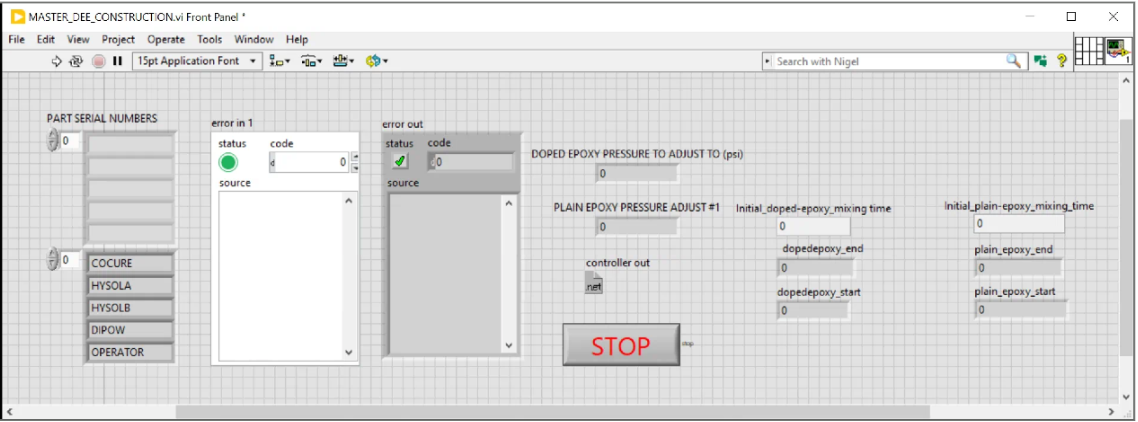
\includegraphics[width=\textwidth]{img2/FrontPanel.png}
\caption{Front Panel of MASTER\_DEE\_CONSTRUCTION.vi}
\label{front_panel}
\end{figure}
\end{center}

\begin{itemize}
    \item Motion Composer: is a program that runs GCODE. GCODE is a set of instructions for the Gantry to move along. Think of a GCODE path like the path a paintbrush needs to be moved along to make a painting.
    %\item For all the GCODE programs, there is a delay of about 5 seconds to allow user to position near the NPaq switch just in case.
    \item Flower Pattern: The cooling tube or evaporator has a flower shape which we call here the flower pattern. The Gantry needs to deposit epoxy while it is moving along the flower pattern path in the Dee. For this, we have a GCODE script/program run by Motion composer.
    \item Carbon fiber-foam co-cure (CFF): The Dee structure is formed by two skins of carbon fiber and two bodies of carbon foam. One carbon fiber skin and carbon foam are co-cured in one entity, so that the Dee is composed of 2 halves of CFF (CFF\_A and CFF\_B). In between the two CFF, inserts and evaporator are sandwiched.    
    \item Insert Filling: Dee has some PEEK inserts that will serve as clamping points for structures/objects on it. The Gantry moves to the location of the insert holes and deposit epoxy while STOPPED at that position. 
    \item Front panel: It is the window through which the user interact with the LabVIEW control program. It shows statistical information, status of the vacuum system, tools and elements in use and other relevant information (see figure \ref{front_panel})
\end{itemize}

%------------------------------------------------------------------
%\section{Responsibilities}

%------------------------------------------------------------------
\section{Equipment}
\begin{center}
\begin{figure}[h!]
    \centering
    \begin{subfigure}[b]{0.45\textwidth}
        \centering
        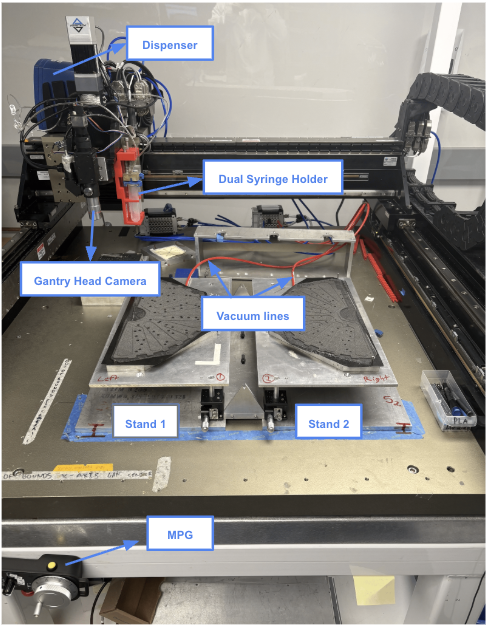
\includegraphics[width=\textwidth]{img2/Gantrysetup.png}
        \caption{Gantry setup. Labels indicate the main parts of the setup.}
        \label{fig:gantry_setup}
    \end{subfigure}
    \hfill
    \begin{subfigure}[b]{0.45\textwidth}
        \centering
        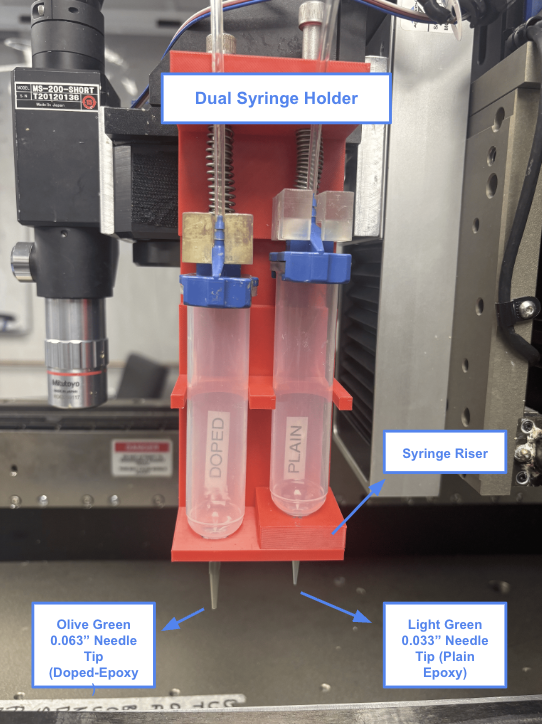
\includegraphics[width=\textwidth]{img2/syringe_holder2.png}
        \caption{Dual Syringe Holder. Labels indicate key attributes of the holder.}
        \label{fig:second_image}
    \end{subfigure}
    \caption{Primary Equipment and Setup for Dee Construction.}
    \label{fig:main_setup}
\end{figure}
\end{center}

\begin{enumerate}

\item Gantry (check that everything (labeled in the figure  \ref{fig:gantry_setup}) is installed and working properly. 
    \begin{itemize}
        \item Syringe holder and riser piece (Figure \ref{fig:second_image})
        \item Stands with alignment screws
        \item Pressurized air Dispenser - Ultimus II
        \item Compressed air lines with splitter
        \item Vacuum manifold and lines
    \end{itemize}
\item Parts and tools
\begin{center}
\begin{figure}[h]
\includegraphics[width=0.45\textwidth,angle = 0]{img2/DEEs.png}
\includegraphics[width=0.45\textwidth,angle = 0]{img/PartsTools_2.png}\\
\includegraphics[width=0.45\textwidth,angle = 0]{img2/Centrifuge.png}
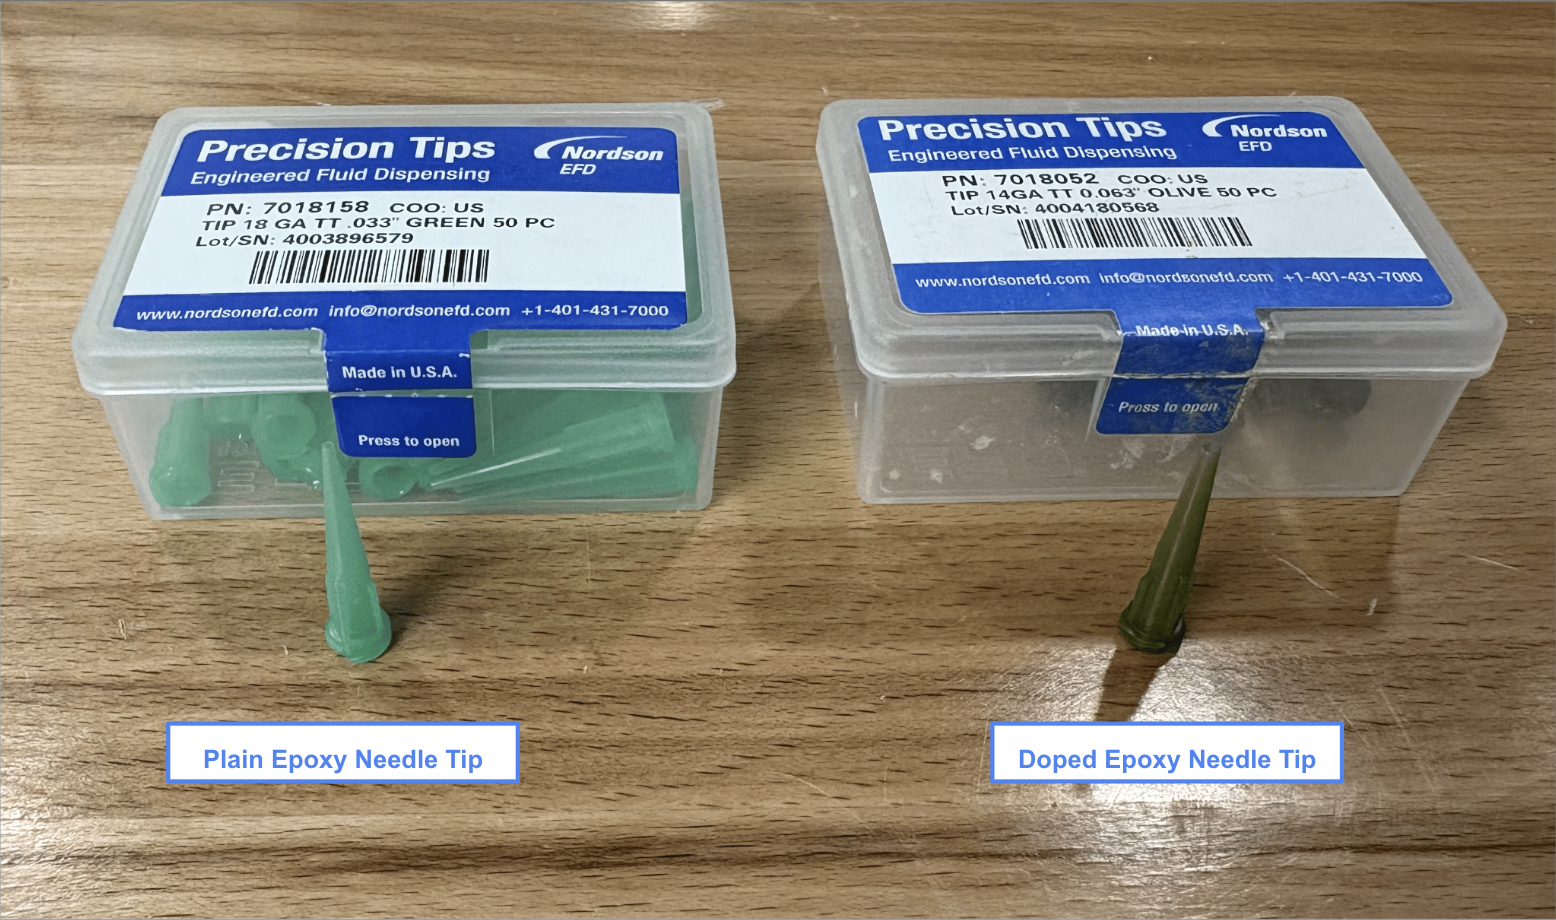
\includegraphics[width=0.45\textwidth,angle = 0]{img2/needle_tips.png}
\caption{Parts and tools used in the DEE manufacturing process. Materials listed for epoxy preparation should be located on the table inside room PSB 375 where the epoxy mixing will be performed; the rest of materials must be located on the table in front of the gantry except for evaporator, inserts and tweezers which should be located on the table left to the gantry.}
\label{Parts ands tools}
\end{figure}
\end{center}
    \begin{itemize}
        \item Side A Half-Dee CFF\_A 
        \item Side B Half-Dee CFF\_B
        \item PEEK Periphery
        \item EA9396 Epoxy  parts A and B. 
        \item Flower-Pattern Shape Titanium $CO_2$ tube/evaporator
        \item 0.063" Olive green Nordson fluid dispensing tip
        \item 0.033" Light green Nordson fluid dispensing tip
        \item Box with PEEK inserts (56 will be used)
        \item Tweezers
        \item Two bottom jig plates (with vacuum lines)
        \item One top jig plate
        \item Both 3D printed tools for sealing tubing and inserts
        \item Flower pattern cover piece (for spreading epoxy)
        \item Small scraping tool for epoxy removal from holes
        \item Neodymium magnets for securing CFF Half-Dee to Jig plate
        \item Small spatula tool
        \item Small soft paint brush
        \item Painter's Tape
    \end{itemize}
\item Epoxy preparation \textbf{(Performed in PSB 375)}
    \begin{itemize}
        \item Small jar of 12-20 Micron Diamond Powder
        \item EA9396 Epoxy Part A
        \item EA9396 Epoxy Part B
        \item 2 Popsicle Sticks
        \item 2 Large Syringes, 2 Pistons, 2 Blue stopper caps
        \item Digital Scale
        \item Centrifuge with Counterweights Installed
        \item Paper Towels
        \item Isopropyl Alcohol
        \item Rubber beakers
        \item Nitrile Gloves
        \item Face Mask
        \item Square plastic sheet
        \item Stopwatch
        \item Box Fan
        \item Painter's Tape
    \end{itemize}
\end{enumerate}
%------------------------------------------------------------------
\begin{figure}[h]
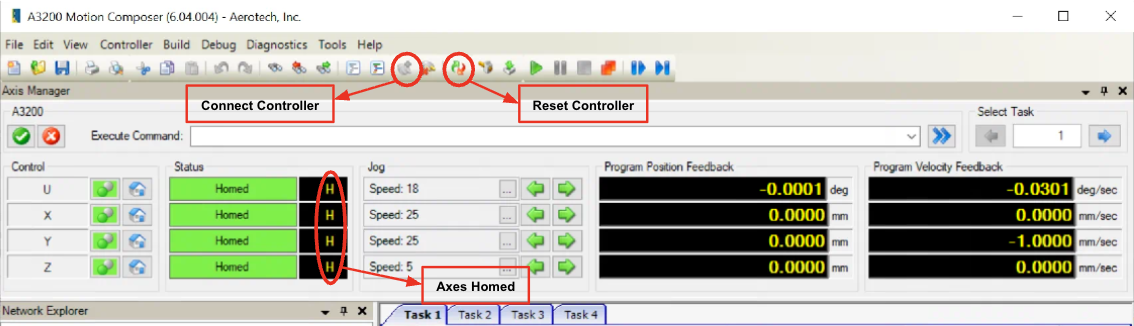
\includegraphics[width=1\textwidth,angle = 0]{img2/motioncomposer.png}
\caption{Motion Composer software used to operate gantry, MPG, and run G-CODE scripts for deposition.}
\label{motion_composer}
\end{figure}

\section{Procedure}
\subsubsection*{Person 1:}
\begin{enumerate}
    %Perform a readiness check of the gantry:
%    \begin{itemize}[leftmargin=*]
    \item Check that the NPaq, power supplies, dispenser and vacuum pumps are turned on. Turn on any if necessary
    \item Check compressed air lines are open
    \item Open LabView control software  \verb|C:\Users\co2_clt\Documents| \verb|\MASTER_DEE_Construction|\\ \verb| \MASTER_DEE_CONSTRUCTION.vi|
    Ensure that it opens in Labview 2025.
    \item Open Motion composer
    \item Check that no other Gscript or Labview programs are running since they can interfere with the deposition.
    \item Make sure in Motion Composer the Gantry is connected as shown in Figure \ref{motion_composer}. The elongated circle should not show VH's (virtual home) but just H's (Home). If VH is shown, the NPAQ is likely turned off.
    \item Ensure the MPG program is running in Motion Composer and check that the MPG is working properly. MPGSample should be running in motion composer and dwelling on \textit{Program Pause}.
    \item Test presence of vacuum and dispenser via test programs in the same folder. 
    \begin{enumerate}
        \item \textbf{Dispenser\_Shot.vi} tests the dispenser
        \item \textbf{manifold.vi} tests the vacuum
    \end{enumerate}
    \item Identify parts. Handle with gloves, face mask. Check that the parts are in good condition.
    \item Assign a new unique Dee number(\texttt{D\_xxx}).
    \item \textbf{Run control program:} \verb|MASTER_DEE_CONSTRUCTION.vi| and provide the information required:
    \begin{enumerate}
        \item Part numbers.
        \item Dee identification.
        \item other required info
    \end{enumerate}
    \item Mount the bottom jig plate onto the stand 1 and align it using the alignment screws (Figure \ref{JigAlignment}).
    \begin{figure}[H]
        \centering
        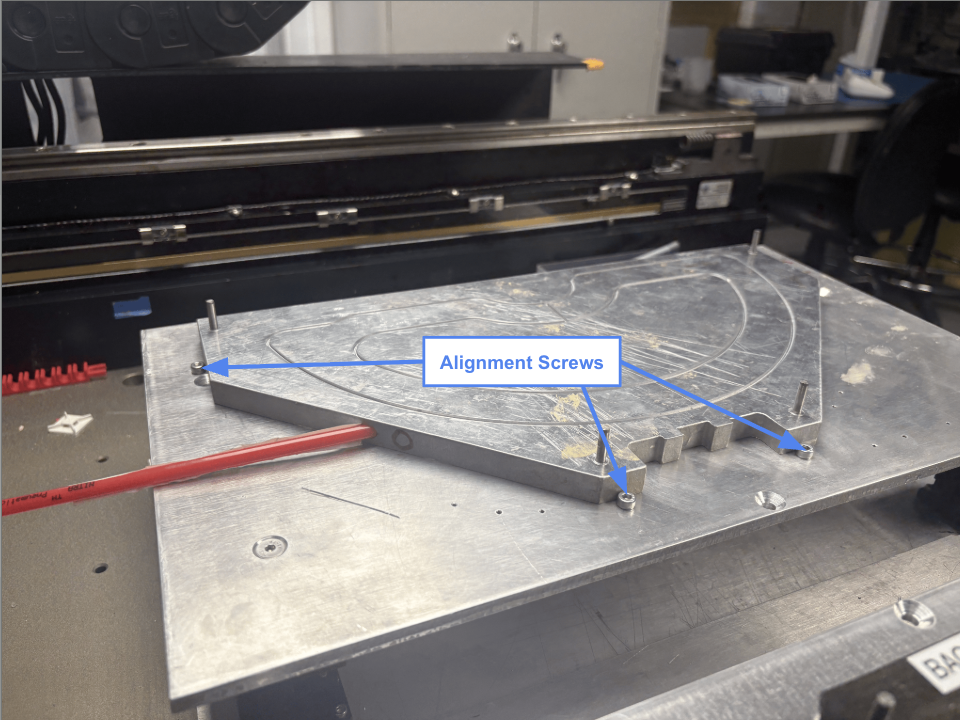
\includegraphics[width=.4\linewidth]{img2/jig_alignment2.png}
        \caption{Jig alignment}
        \label{JigAlignment}
    \end{figure}
    \item Connect labeled vacuum line to corresponding bottom jig.
    \item Mount the CFF\_A onto the bottom jig plate on Stand 1 using the jig poles and holes in the CFF\_A.
    \item For CFF\_B mount it on bottom jig plate and put it on person 2 working table for now. When deposition for CFF\_A finish and before starting deposition for CFF\_B put it with the bottom jig plate on stand 2. Make sure to connect labeled vacuum line to corresponding bottom jig.
    \item Use the neodymium magnets to secure the CFF halves onto the jig plates. Place them around the edges of the CFF halves. The magnets should lock into the correct positions.
\begin{figure}[H]
    \centering
    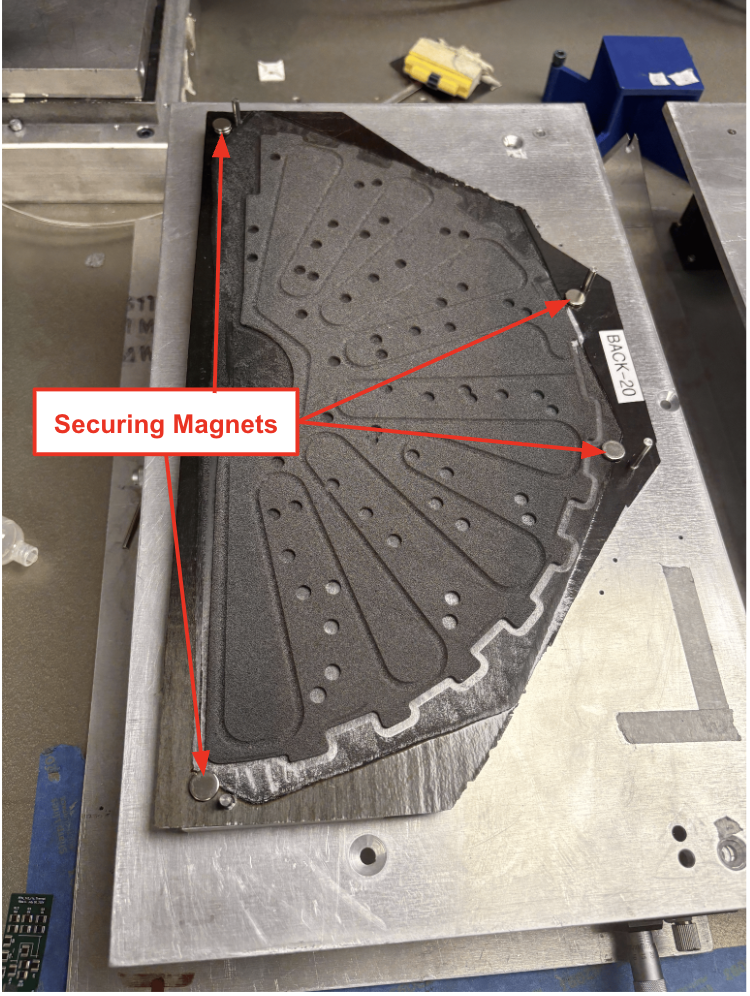
\includegraphics[width=0.4\linewidth]{img2/Magnets2.png}
    \caption{Neodymium magnets used to secure CFF halves onto the jig plates.}
    \label{magnets}
\end{figure}
    %Gantry Loading, calibration and epoxy deposition
%    \begin{itemize}[leftmargin=*]
        \item After person 2 comes into the clean room with both syringes and the container of doped epoxy, the control program will have moved the gantry up to the front of the table awaiting syringe installation. Screw the blue pressure cap and hose assembly onto the syringes.
        \item Unscrew the blue stopper cap at the bottom of the both syringes, install the \textit{olive green 0.063"} needle tip onto the doped-epoxy syringe AND the \textit{light green 0.033"} needle tip onto the plain epoxy syringe and load both syringes into their designated positions on the dual syringe holder.
        \item Use the dispenser pressure foot pedal and pressure splitters to bring the epoxy of each syringe to fill the tip so that there are no air bubbles in the syringe tips initially. Use a pressure $\leq 5.5$ PSI for the plain epoxy syringe and a pressure $\leq 40.0$ PSI for the doped epoxy syringe. Wipe off any epoxy from the tips. Select "Okay" when both syringes are installed and no air bubbles remain in the syringe tips. 
       \item \textit{Initially}, the unused plain epoxy syringe should be elevated and the compressed air splitter should be open for doped epoxy (See Figure \ref{fig:second_image}).
        \item The program will send the gantry home, and the user will be prompted once more before the flower pattern deposition begins. Select "Proceed" once you perform the final checks listed on the front panel prompt and the gantry will moved to the start of the flower pattern.
        \item \textbf{*Ensure that you know the exact times that person 2 began mixing both epoxies* The elapsed times since the mixing of each will be used in the programs flow.}
        \item Check that the olive needle tip is in the starting point for epoxy deposition as shown in figure \ref{needleref}. It should sit directly over the start of flower pattern line. If needle tip is not in position, adjust it using the MPG.
        \begin{figure}[H]
            \centering
            \includegraphics[width=0.45\linewidth]{img2/FPATstart1.png}
            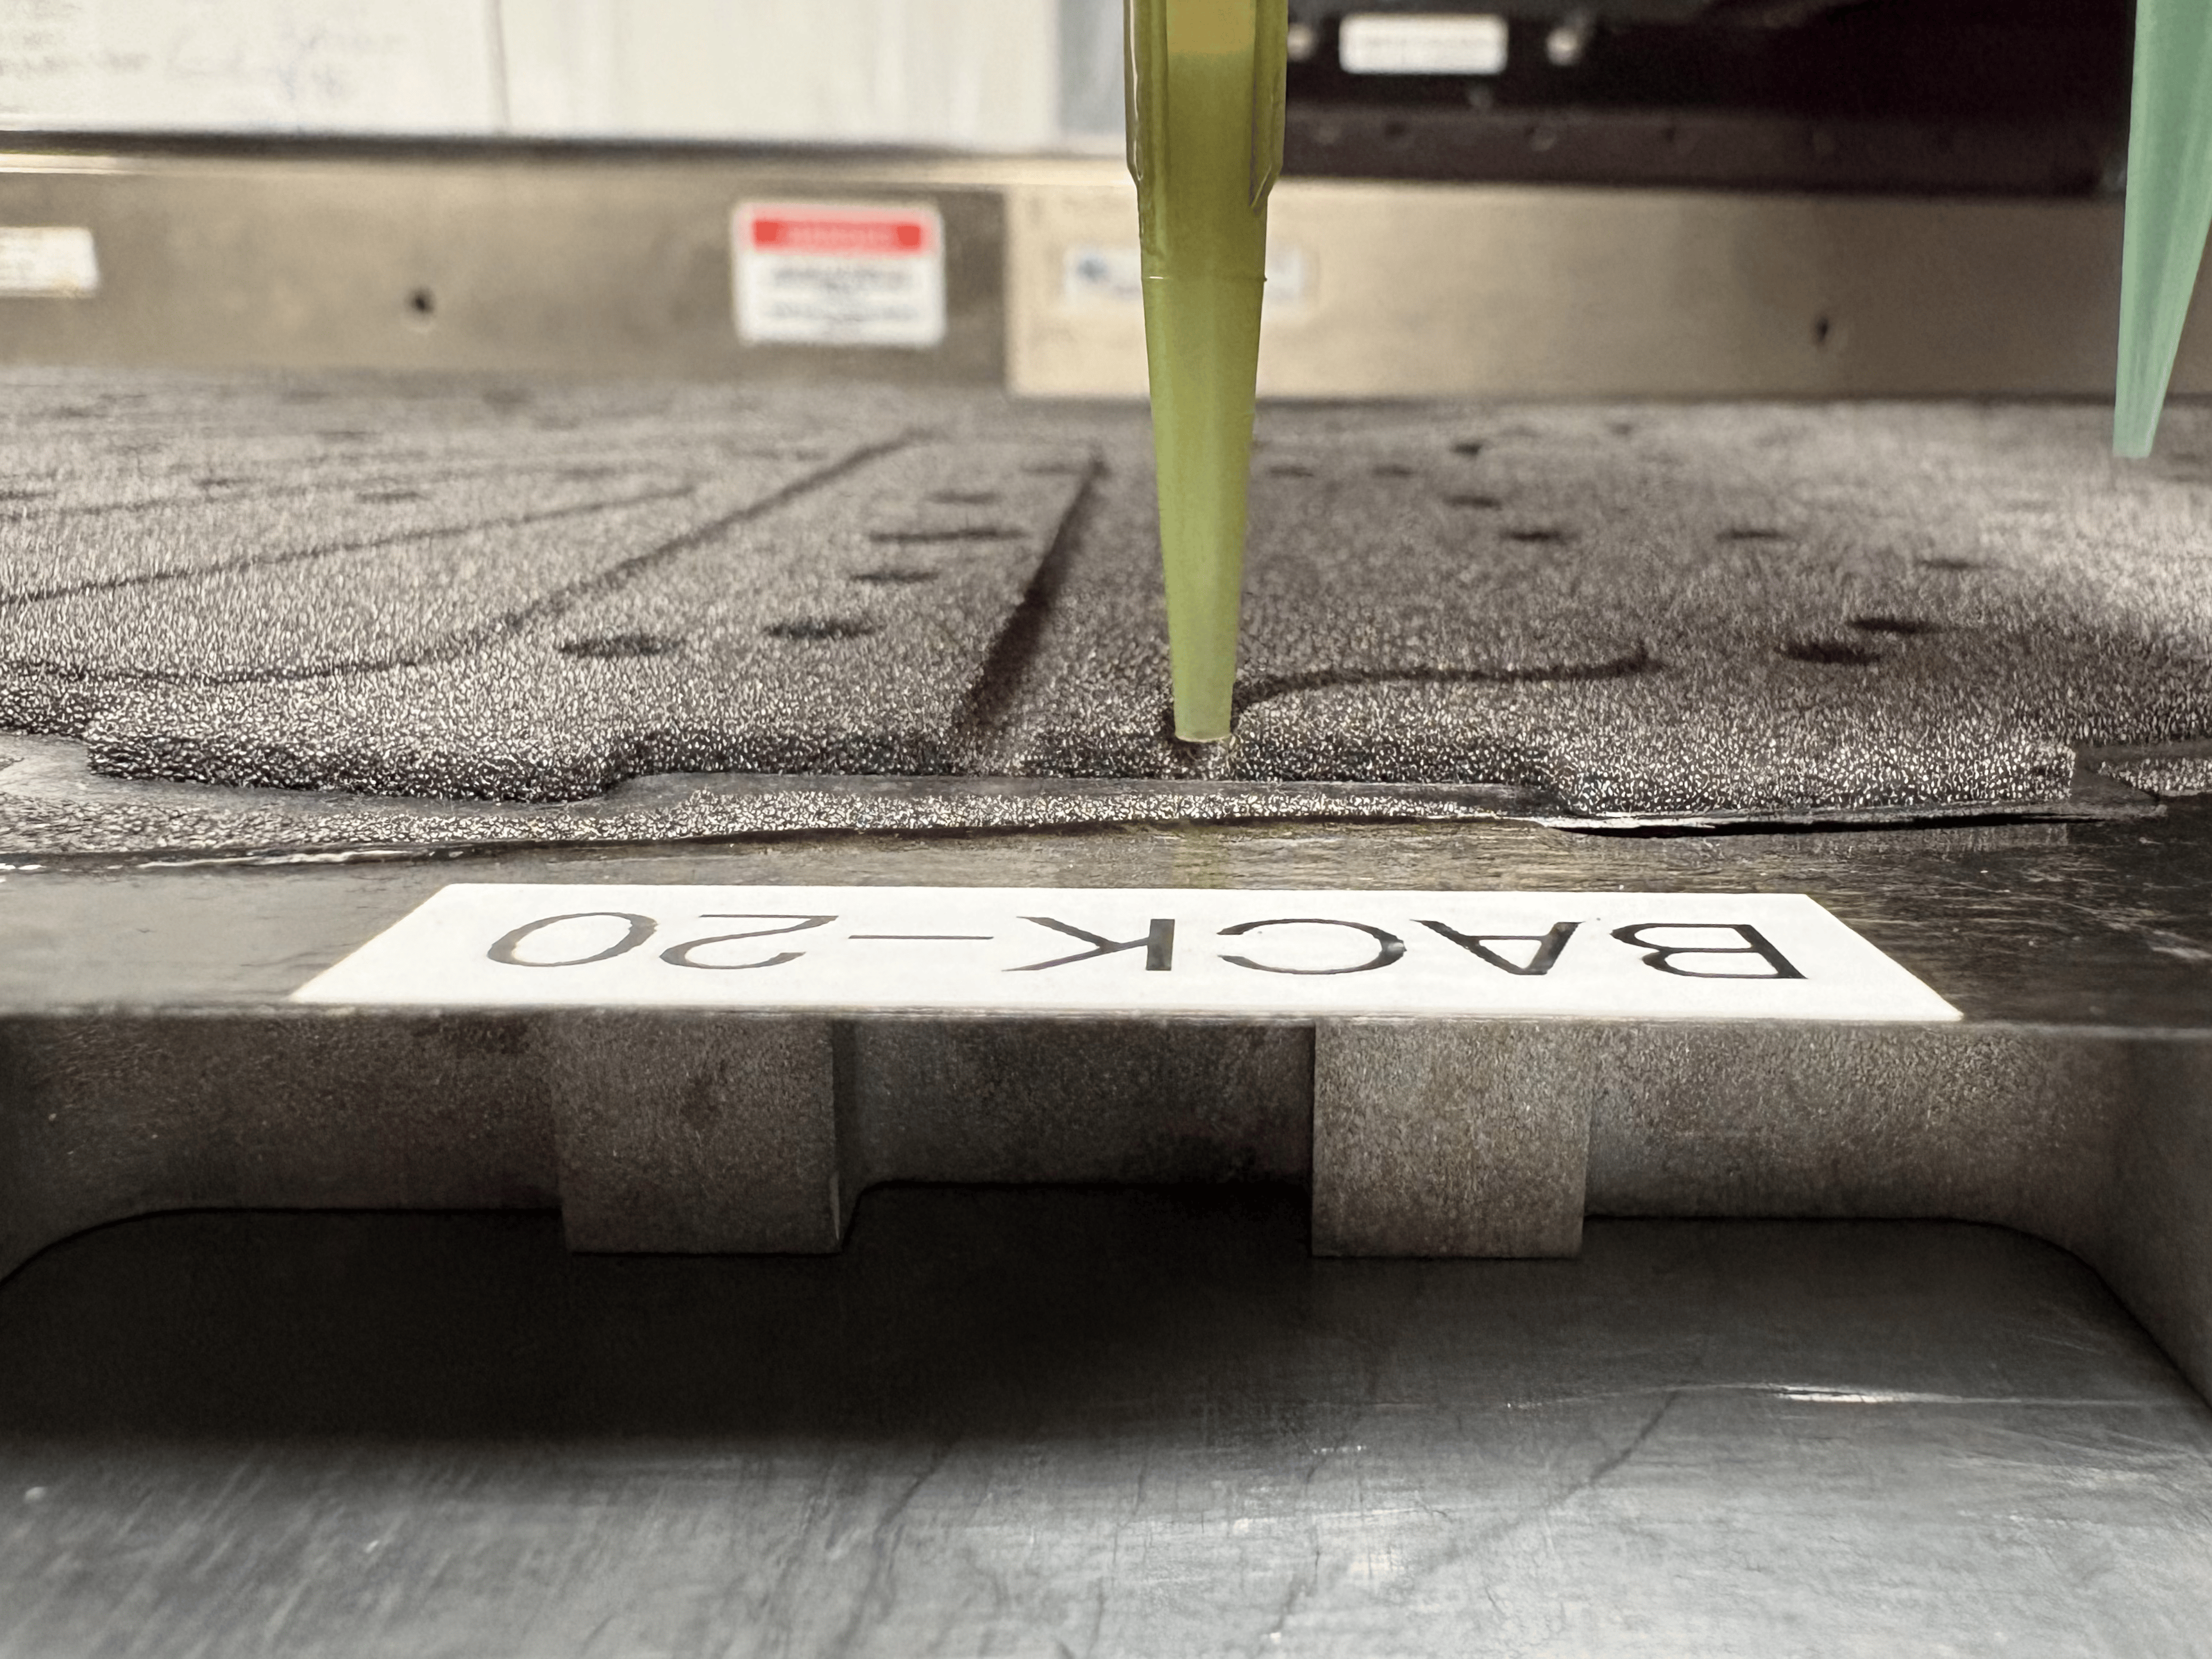
\includegraphics[width=0.45\linewidth]{img2/FPATstart2.png}
            \caption{Needle starting position}
            \label{needleref}
        \end{figure}
        \item \textbf{[Flower Pattern Side A]} When prompted, enter the integer amount of time that has elapsed since the doped-epoxy had been mixed. Adjust pressure to the output amount provided. Begin flower pattern doped epoxy deposition by selecting "OK" for the pressure adjust in the front panel of LabView program. Check for consistent epoxy flow and adjust the pressure if needed during the deposition.
        \item \textbf{[Filling Side A]} After the flower pattern is completed, use the splitters to switch the compressed airflow to the plain epoxy syringe. Elevate the doped-epoxy syringe. When prompted enter the integer amount of elapsed time since plain epoxy was mixed, adjust the pressure accordingly. Ensure that the light green needle tip is aligned directly over the first hole in the filling deposition (adjust via MPG if not aligned) and select "OK" to proceed with Filling deposition.
        \item \textit{When each deposition ends on CFF\_A, get up and check the deposition to make sure it's enough. You will be prompted on whether you would like to repeat the process of deposition for each step (Flower Pattern/Filling). If it's not enough, simply rerun the deposition ON TOP OF that deposition for CFF\_A and select and YES. If it is enough, select NO. After continuing, the gantry will move to starting point for periphery deposition.}  
        \begin{figure}[H]
            \centering
            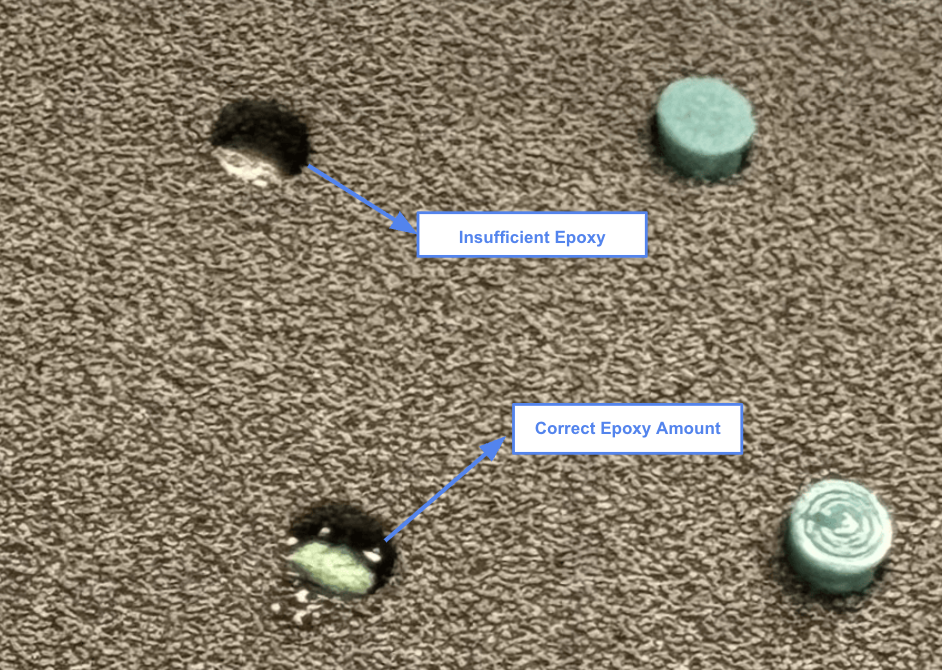
\includegraphics[width=\linewidth]{img2/Epoxy_fillings.png}
            \caption {Plain epoxy filling hole examples}
            \label{epoxyref}
        \end{figure}
        \item \textbf{[Periphery Side A]} Increase the pressure used in the prior filling deposition step by 1.0 PSI. \textit{The start position should be just in front of the beginning of flower pattern deposition on the border encompassing the carbon foam.} Adjust position with the MPG if needed. Select "OK" to begin depositing plain epoxy around the edges of CFF\_A.
        \item After the periphery deposition ends, the gantry head will move out of the way of CFF\_A. Remove CFF\_A from the gantry table and hand to person 2
        \item At this time person 2 is supposed to have finished with CFF\_B so take the CFF\_B with the buttom jig plate and mount it on stand 2. Remeber to connect vacuum line.
        \item Before deposition for CFF\_B, make sure to hand over CFF\_A to Person 2, who will do the PEEK periphery, inserts, and flower pattern tubing installations.
        \item Switch the compressed air splitter back to doped-epoxy and elevate the plain epoxy syringe
        \item Check that the needle tip is in the starting point for flower-pattern doped epoxy deposition. Adjust position accordingly and \textbf{adjust pressure} according to the front panel pop-up.
        \item \textbf{[Flower Pattern Side B]} Begin epoxy deposition by hitting OK button in the front panel of LabView program. Check for consistent epoxy flow.
        \item \textbf{[Filling Side B]} Switch the splitter to plain epoxy and elevate the doped-epoxy syringe. Adjust starting position with MPG if needed. Adjust pressure according to the front panel pop-up and select "OK" to begin filling deposition.
        \item \textit{When each deposition ends on CCF\_B, get up and check the deposition to make sure it's enough. You will be prompted on whether you would like to repeat the process of deposition for each step. If it's not enough, simply adjust the pressure to what you want to deposit ON TOP OF that deposition for CCF\_B and select and YES. If it is enough, select NO.}
        \item \textbf{[Periphery Side B]} Increase the pressure used in the prior filling deposition step by 1.0 PSI. Ensure proper starting position alignment. Select "OK" to begin depositing plain epoxy around the edges of CFF\_B.
        \item Remove CFF\_B from the gantry table and bring to person 2, who should be finished (or almost finished) pressing the filling inserts, periphery, and evaporator tubing into CFF\_A
        \item Flip CFF\_B so that carbon foam face towards the floor.
        \item Use poles on bottom jig to stack CFF\_B on top of CFF\_A.
        \item stack top jig plate on top of CFF\_B. Make sure all of the pieces fit into place and holes are aligned when joined together.
        \item Take the full stack into the oven; turn on the oven and let bake for 2 hours @ 50C, with 4h cooling. Follow instructions fixed on the oven door as shown in Figure \ref{oven}. 
        \item Clean up the working space.
        \begin{figure}[h]
            \centering
            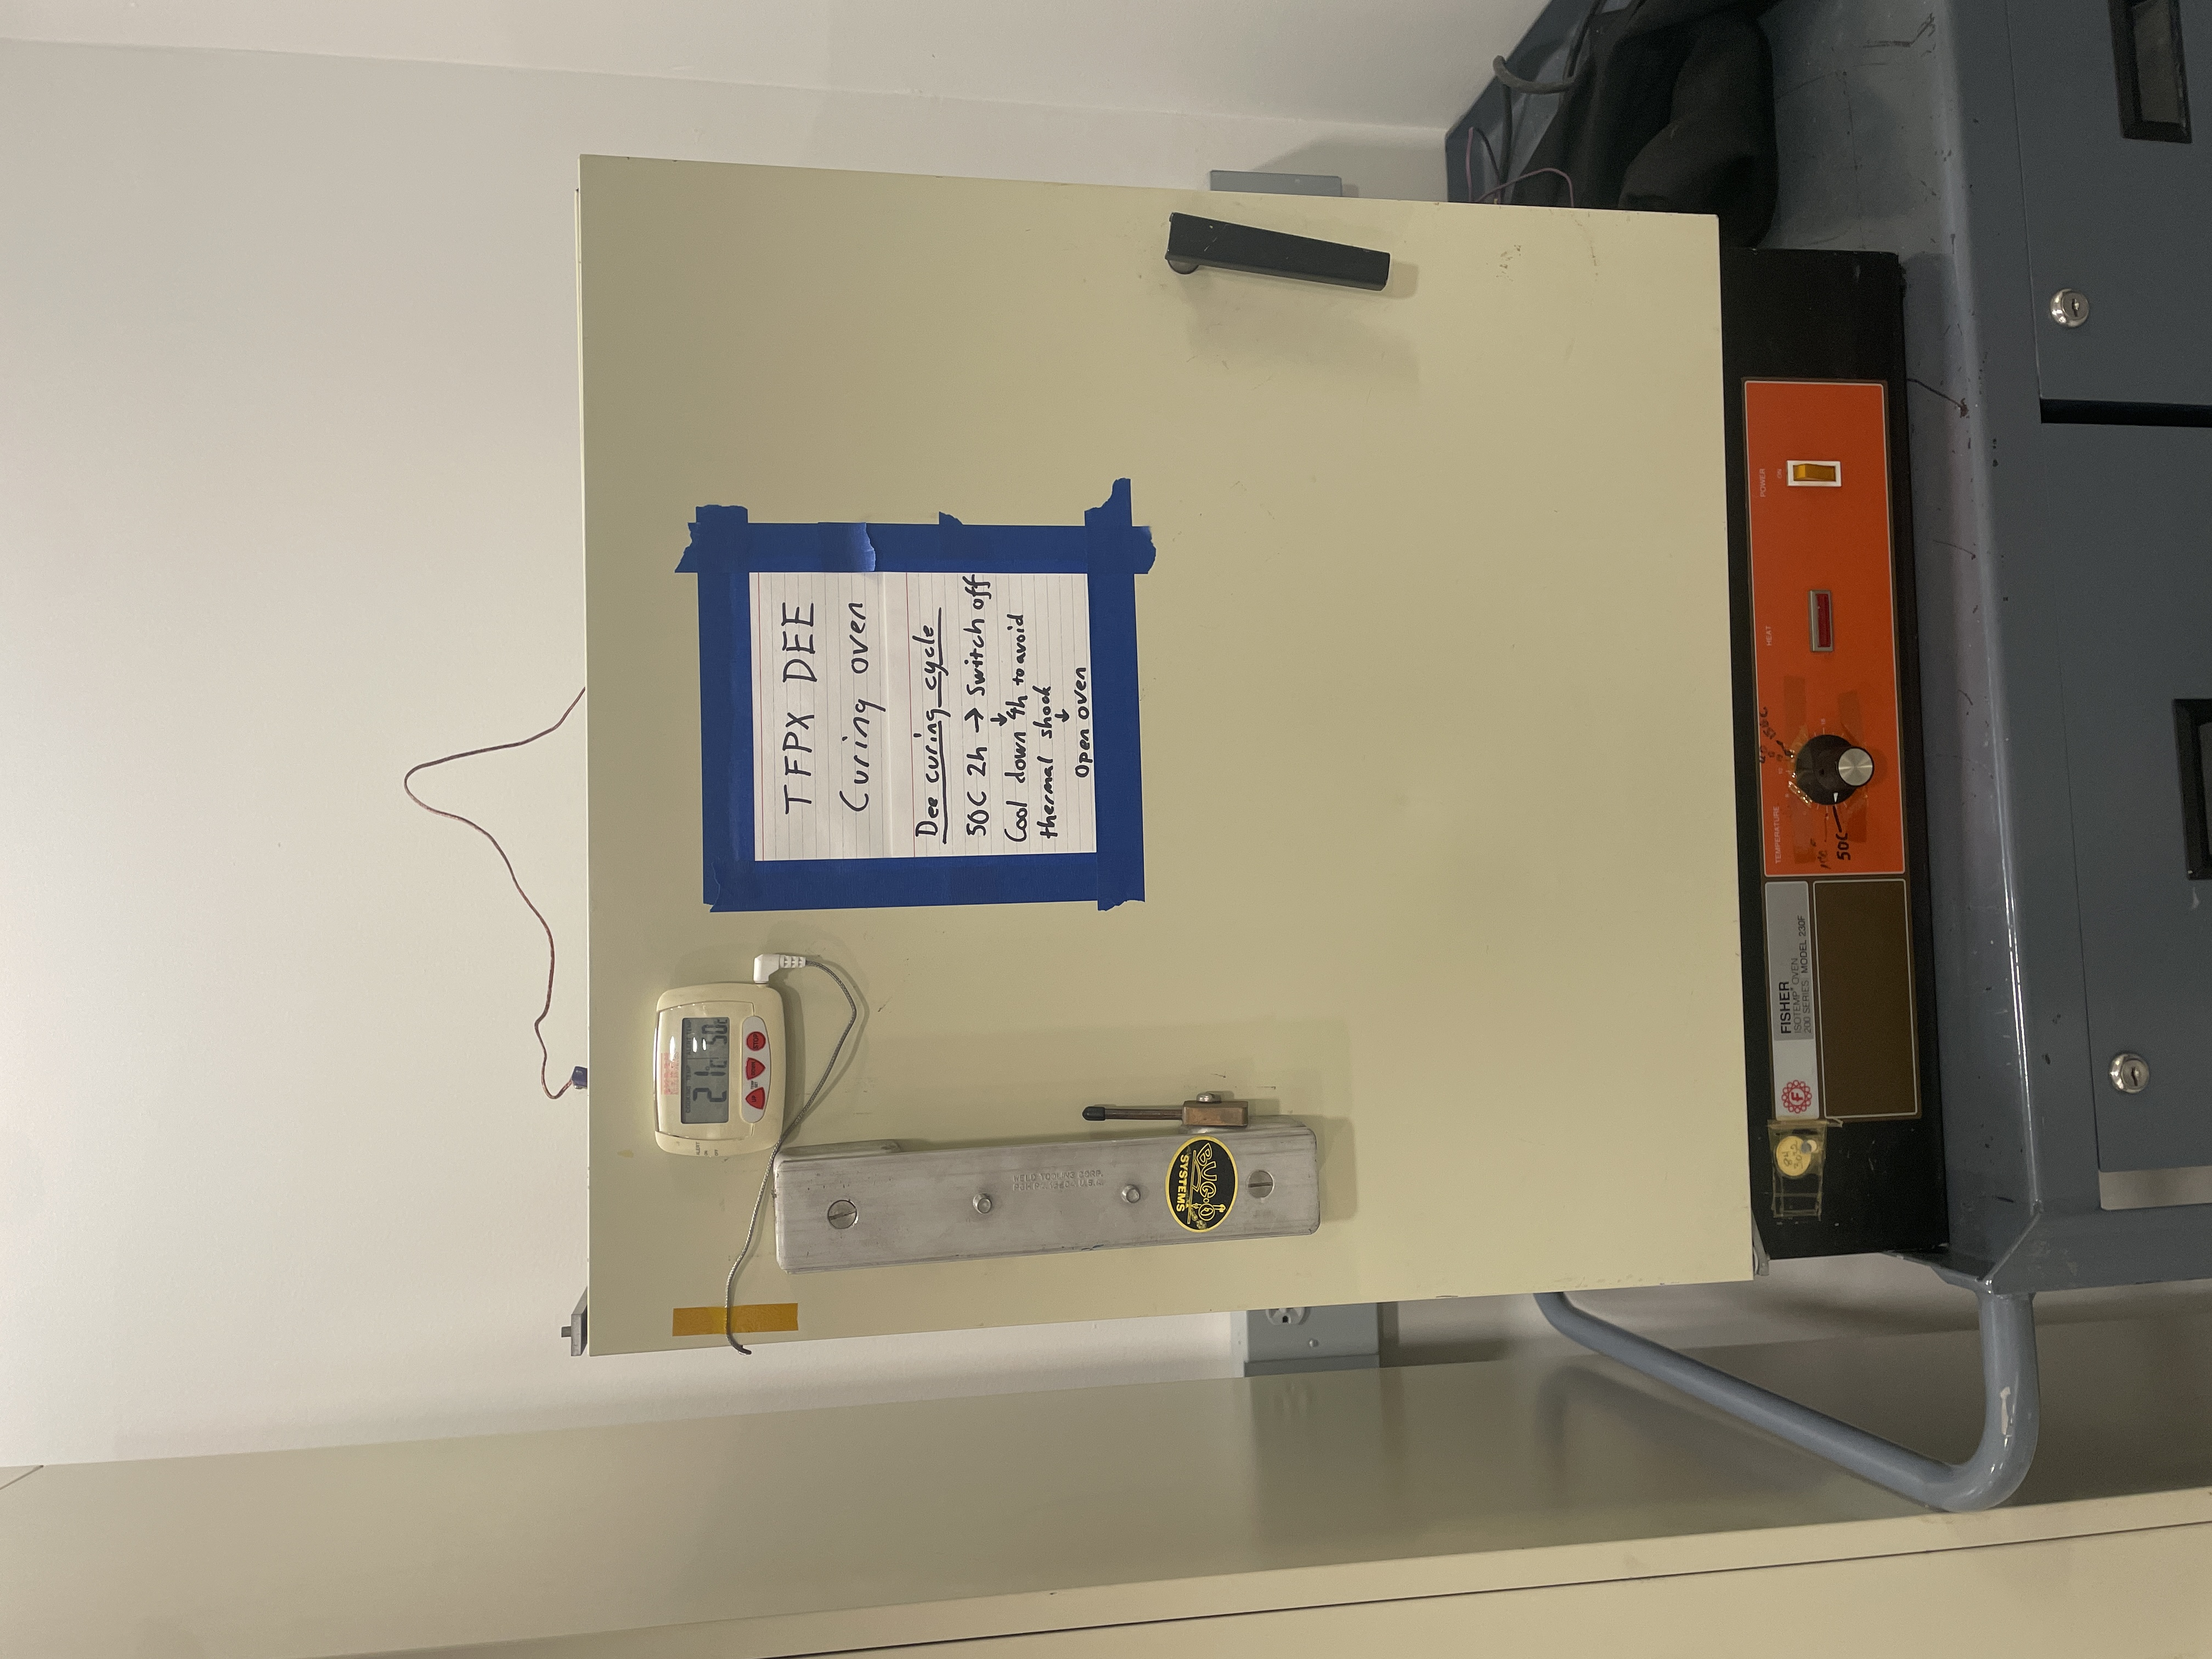
\includegraphics[width=0.4\linewidth, angle=-90]{img/oven.JPG}
            \caption{Oven for curing Dee after assembly}
            \label{oven}
        \end{figure}

\end{enumerate}   
\newpage
\subsubsection*{Person 2:}
\begin{enumerate}
    %Perform a readiness check of epoxy \\preparation area:
%   \begin{itemize}[leftmargin=*]
        \item Ventilate the room with the fan
        \item Put on a face mask and gloves. Lay out paper towels over the table and tape it.
        \item Materials are on the table.
        \item Turn scale on in units of grams.
        \item Check that centrifuge is ready to use.        
%    \end{itemize}      
    %\item Epoxy Mixing and Syringe Preparation
%    \begin{itemize}[leftmargin=*]
        \item Determine the amount of epoxy to be prepared using table in figure for the syringe with doped epoxy (Figure \ref{fig:epoxy_calc}).
        A calculator has been set up \href{https://cornellprod.sharepoint.com/:x:/r/sites/TFPXDeemanufacturing/_layouts/15/Doc.aspx?sourcedoc=%7B1955F9BA-B34C-40AF-83B5-E2F571FD91B1%7D&file=Epoxy%20mixing%20calculator.xlsx&action=default&mobileredirect=true}{here} in case a different amount of epoxy is desired. 80g of doped-epoxy and 20g of plain-epoxy is used as reference in the following.
            \begin{center}
            \begin{figure}[h!]
                \centering
                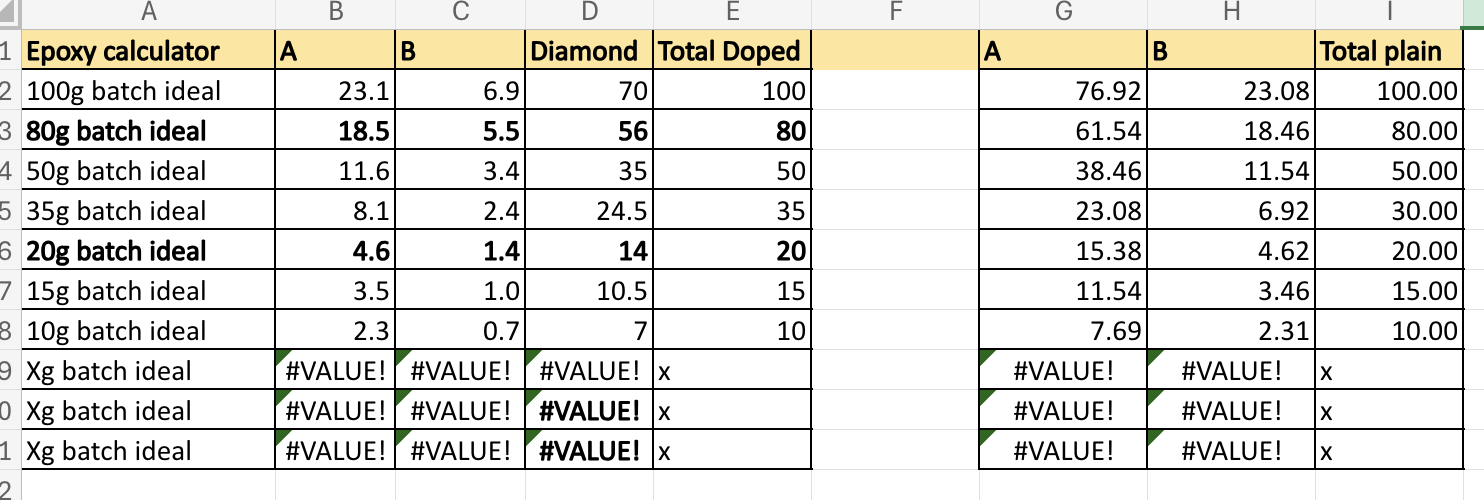
\includegraphics[width=0.9\linewidth]{img/epoxy_calc.png}
                \caption{Epoxy calculator table}
                \label{fig:epoxy_calc}
            \end{figure}
        \end{center}
        \item Place the first beaker (Beaker \#1) on the scale and zero the scale. Add ~18.5g of EA9396 Part A using one side of the Popsicle stick. Remove the beaker from the scale temporarily.
        \item Place the second beaker (Beaker \#2) onto the scale and zero the scale again. Add ~4.6g of EA9396 Part A into beaker \#2 on the scale using the same stick left the beaker on the scale.
        \item Zero the scale and using a clean popsicle stick, place ~1.4g Part B into beaker \#2 then mix immediately. \textbf{Take note of the time at which the plain epoxy is mixed.}
        \item \textit{Communicate with Person 1 the starting times of both plain and doped epoxy.}   
        \item Pour as the mixed plain epoxy solution from beaker \#2 into the syringe and prepare it with the blue cap for the centrifuge.
        \item Before using the centrifuge, weight the plain epoxy syringe and put a counterweight syringe for it on the opposite site in the centrifuge.
        \item Press the start button on the centrifuge and run it. Ensure no weird noises come from the centrifuge, if so, the counter weight is not correct. Ensure no bubbles remain. If so, repeat centrifuging.
        \item Place beaker \#1 back onto the scale. 
        \item Zero the scale again. Add 5.5g of Part B using the other side of the stick.   
        \item Zero the scale one more time. Add 56g of diamond powder and mix until a uniform grayish-green consistency is achieved.  \textbf{Also take note at this time which the doped epoxy is mixed.}
        \item Prepare the syringe, trying to leave 45g on the beaker \#1 for spreading on top the carbon foam of CFF\_B. Don't forget to put the blue tip cap before centrifuging. Transfer the mixed epoxy into the syringe, ensuring minimal loss.
        \item Before using the centrifuge, weight the doped epoxy syringe and put a counterweight syringe for it on the opposite site in the centrifuge.
        \item Press the start button on the centrifuge and run it. Ensure no weird noises come from the centrifuge, if so, the counter weight is not correct. Ensure no bubbles remain. If so, repeat centrifuging.
        \item Push the white plastic piston down onto both syringes using a sharpie/pen, making sure that the trapped air is removed. 
        \item If needed pour xg of dope epoxy until a total of 45g into beaker \#1 by pushing the piston down.
        \item Take both the plain and doped epoxy filled syringes along with beaker \#1 holding the extra doped epoxy to the clean room. Pass them to Person 1.
        \item Get dressed to get into the clean room   
%    \end{itemize}
    %Evaporator and inserts installation
%    \begin{itemize}
        \item Prepare inserts and Evaporator on the working table.
        \item \textbf{[Epoxy Spreading]} While deposition for CFF\_A is running, you should have CFF\_B on the working table. Place the flower pattern cover piece over the CFF\_B flower pattern grooves. Use the Beaker \#1 with doped epoxy and scrape/spread it across the carbon fiber surface of CFF\_B with the plastic scraper tool. 
        \item Clean out the doped-epoxy inside the filling holes (caused by the spreading) using the small spatula tool. After the holes are cleaned, remove the flower pattern cover from CFF\_B.
        \item Put CFF\_B on the stand 2 after the depositions on CFF\_A are completed, BEFORE the start of CFF\_B depositions
        \item Before the epoxy deposition on stand 2 starts, move bottom jig from stand 1 to working table on the left of gantry. 
        \item If needed, use a brush to spread the deposited plain epoxy evenly around the edges where the PEEK periphery will be placed
        \item Glue the Periphery to CFF\_A. Put some pressure around the periphery to ensure bonding. Use your hand/fingers.
\begin{figure}[H]
    \centering
    \includegraphics[width=0.4\linewidth]{img2/pressingpieces.png}
    \caption{Pieces used for pressing inserts and evaporator into Dee}
    \label{fig:pressing}
\end{figure}
        \item Take inserts and stick them on the  CFF\_A carbon foam holes using the red 3D printed tools to press in (Figure \ref{fig:pressing}). Be careful not to break/damage the carbon foam, although some small reshaping of the edges is acceptable as long as the fit is snug.
        \item Insert the evaporator into the groove making sure that it fits. Push in with the red pressing tools.
        \item Prepare top jig plate to complete the full stack.
        \item Clean up the working space and all materials used. Use isopropyl alcohol to clean out the beakers and the wipes to clean all surfaces and tools.
                                         
\end{enumerate}
%------------------------------------------------------------------
\section{Documentation}

Any special observations, e.g. damage to parts not already recorded during visual inspection, deviations from normal procedures, should be added to the report in the last step of the routine in the comments pop-up window 

The following information is recorded in the report generated by the gluing software:
\begin{itemize}
    \item Date, time (start--end) and operator name
    \item LabView software: version
    \item Id of parts used:
	\begin{itemize}
	    \item Carbon fiber-foam: S/N
	    \item Dee ID
	    \item Epoxy information
	\end{itemize}
    \item observations/comments
\end{itemize}

Find the report at \\ \verb| C:\Users\co2_ctl\Documents\Final_Dee_Assembly\Dee_Assy_Reports\Report.xls|.\\ Write an ELog entry and upload the report to it and to the appropriate DataBase.  

\end{document}

